\documentclass{article}
\usepackage[top=.5in, bottom=1in, left=0.75in, right=0.75in]{geometry}
\usepackage{graphicx}

\title{Numerical Linear Algebra Program Assignment 3a Report}
\author{Hunter Garrison}
\date{Due: March 29, 2024 @ 11:59PM}

\begin{document}

\maketitle  % This command generates the title, author, and date

\section*{Task 1}
\subsubsection*{Algorithm 1}
The purpose of Algorithm 1 is to solve the linear least squares using household reflectors to convert a matrix $A$ to form $R$ 
(an upper right triangular matrix). Upon doing this, we can multiply the same household reflectors against a vector $b$ in order to find
the solution to our problem.\newline\newline
We begin by testing our algorithm on square nonsingular matrices with sizes ranging from 10 to 200 showing relative error vs. 
matrix size, $n$. The relative error is compared against the np.linalg.lstsq method as "true x".\newline
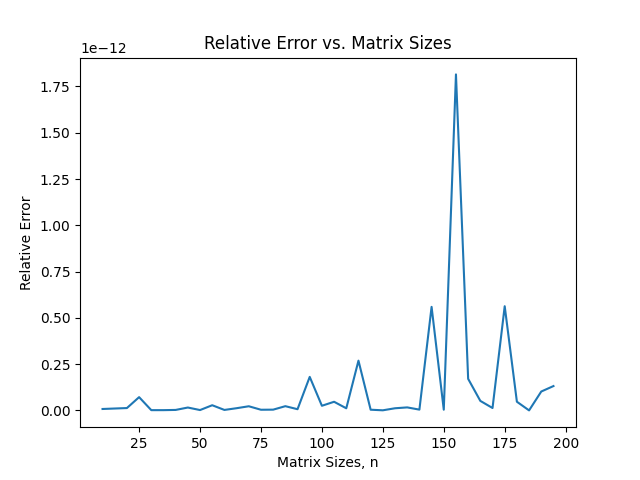
\includegraphics[width=\linewidth]{Images/Figure_1.png}\newline
We see that as our matrix size increases, we start to get more and more unstable errors, which is expected.\newline\newline
We now test our algorithm on rectangular full column rank matrices $A$ such that $n > k$ and $b\in\mathcal{R}(A)$.\newline
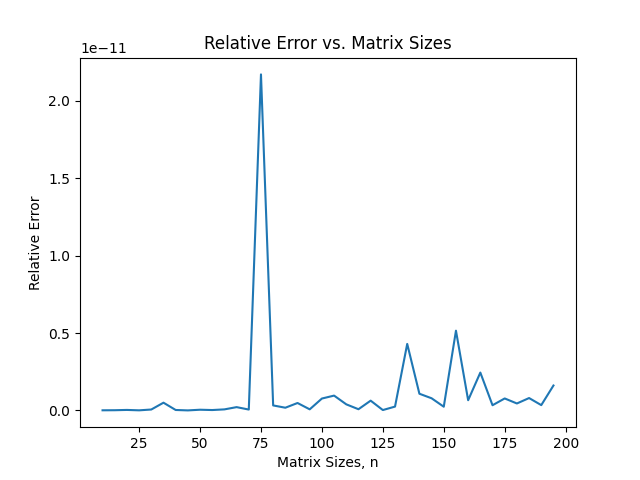
\includegraphics[width=\linewidth]{Images/Figure_2.png}\newline
We see that we have a few spikes, but for the most part our errors are low.\newline\newline
Finally, our last test is on rectangular full column rank matricies $A$ such that $n>k$ and $b\notin\mathcal{R}(A)$ and $b=b_1+b_2$ 
where $b_1\in\mathcal{R}(A)$ and $b_2\notin\mathcal{R}(A)$ that define a linear least squares problem with a nonzero 
residual $r_{\min} = b_2 = b-Ax_{\min}$.\newline
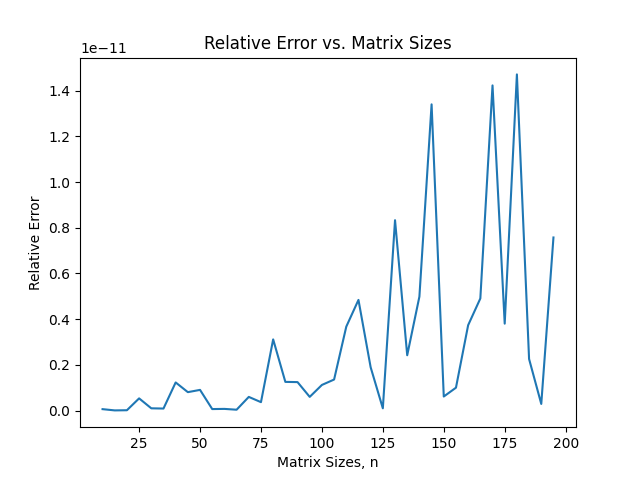
\includegraphics[width=\linewidth]{Images/Figure_3.png}\newline
We see that our results are similar to those from test 1, with the larger matrix sizes resulting in larger relative errors.
\subsection*{Algorithm 2}
Our second algorithm is performing the incremental least squares approach to find $x_{min}$. We generate random matrices of size n=2 to n=200 
and plot the relative errors errors below. \newline
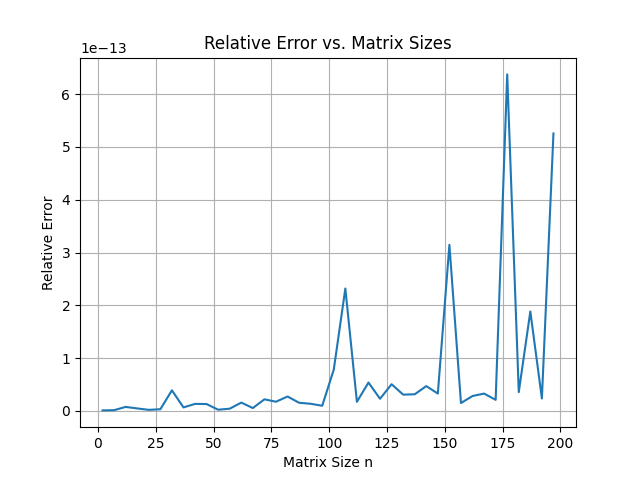
\includegraphics[width=\linewidth]{Images/Figure_4.png}\newline
We see that similar to our other algorithm, our errors are starting to get unstable as the size of the matrix increases.\newline

\section*{Task 2}
Our second task is to consider the regularizes linear least squares described in the program assignment details. Below is the sinusoid 
showing all combinations of different $\lambda$ and $n$ values.\newline
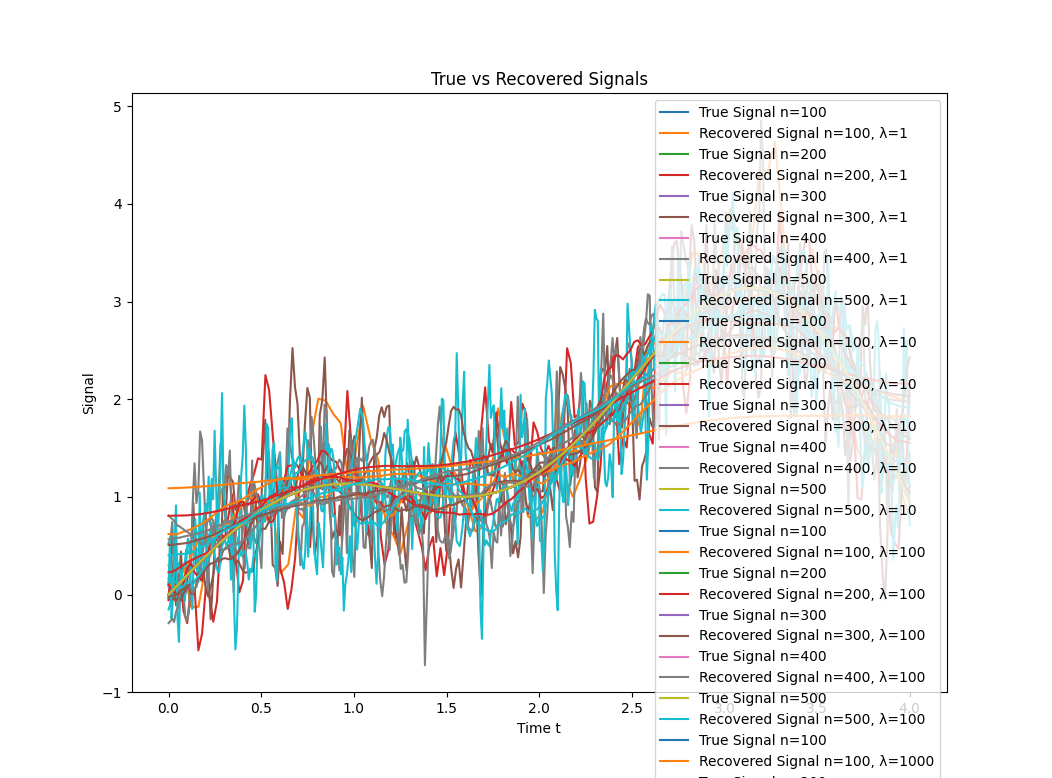
\includegraphics[width=\linewidth]{Images/Figure_5.png}\newline




\end{document}